\chapter{Atividade 6 -- Integral pelo método do trapézio: sincronização em OpenMP}

\label{chap:atvd06}

\section{Enunciado da tarefa}

\label{sec:atvd06-enunciado}

\begin{quote}

Implemente diferentes versões de um programa para o cálculo de integrais
definidas utilizando o método do trapézio.

O programa deve permitir calcular numericamente a integral de uma função
\(f(x)\) em um intervalo \([a,b]\), utilizando \(n\) subdivisões.

Devem ser implementadas as versões sequencial, paralela sem tratamento para
região crítica, paralela utilizando \texttt{critical}, paralela utilizando
\texttt{atomic} e paralela utilizando \texttt{reduction}.

Após a implementação, compare os resultados obtidos e os tempos médios de
execução de cada versão à medida que o número de subdivisões \(n\) aumenta.
Utilize gráficos para apresentar e analisar os resultados.

\end{quote}


\section{Objetivos e requisitos}

\label{sec:atvd06-objetivos}

A Atividade 6 constitui uma extensão direta da Atividade 4. Na atividade
anterior, o método composto do trapézio foi implementado sequencialmente e
a estrutura do algoritmo foi analisada quanto às possibilidades de
paralelização. Nesta atividade, essas possibilidades foram efetivamente
implementadas utilizando OpenMP.

O principal objetivo foi avaliar experimentalmente diferentes formas de
tratar a variável acumuladora existente no método do trapézio quando o
laço principal é executado por múltiplas threads.

Foram implementadas cinco versões:

\begin{enumerate}
    \item implementação sequencial;
    \item implementação paralela sem sincronização;
    \item implementação paralela utilizando \texttt{critical};
    \item implementação paralela utilizando \texttt{atomic};
    \item implementação paralela utilizando \texttt{reduction}.
\end{enumerate}

Os principais requisitos experimentais foram:

\begin{itemize}
    \item manter o mesmo problema matemático utilizado na Atividade 4;
    \item utilizar \texttt{int64\_t} no cálculo numérico;
    \item variar apenas o número de subdivisões \(N\);
    \item manter fixo o número de threads;
    \item utilizar o mesmo escalonamento nas versões paralelas;
    \item medir o tempo médio de execução;
    \item validar a correção das versões sincronizadas;
    \item registrar, sem interromper o experimento, os erros da versão sem
    sincronização;
    \item calcular o speedup em relação à implementação sequencial;
    \item produzir dados adequados à construção de gráficos;
    \item analisar o impacto de sincronização, contenção e redução sobre o
    desempenho.
\end{itemize}


\section{Fundamentação conceitual}

\label{sec:atvd06-fundamentacao}

\subsection{Método composto do trapézio}

O problema numérico permaneceu o mesmo da Atividade 4. Uma integral definida

\begin{equation}
    I = \int_a^b f(x)\,dx
\end{equation}

é aproximada dividindo-se o intervalo \([a,b]\) em \(N\) subdivisões de
largura

\begin{equation}
    h = \frac{b-a}{N}.
\end{equation}

Os pontos da discretização são

\begin{equation}
    x_i = a + ih,
    \qquad i=0,1,\ldots,N.
\end{equation}

A formulação utilizada na implementação foi

\begin{equation}
    I_N =
    h
    \sum_{i=1}^{N-1} f(x_i)
    +
    \frac{
        h[f(a)+f(b)]
    }{2}.
    \label{eq:atvd06-trapezio}
\end{equation}

A função utilizada foi

\begin{equation}
    f(x)=x^2
\end{equation}

no intervalo

\begin{equation}
    [a,b]=[0,2\,400\,000].
\end{equation}

A integral exata é

\begin{equation}
    I_{\text{exato}}
    =
    \int_0^{2\,400\,000}x^2\,dx
    =
    \frac{(2\,400\,000)^3}{3},
\end{equation}

resultando em

\begin{equation}
    I_{\text{exato}}
    =
    4\,608\,000\,000\,000\,000\,000.
    \label{eq:atvd06-integral-exata}
\end{equation}


\subsection{Erro numérico}

Para \(f(x)=x^2\), o erro do método composto do trapézio pode ser
determinado exatamente por

\begin{equation}
    E_N =
    \frac{(b-a)h^2}{6}.
    \label{eq:atvd06-erro}
\end{equation}

Como \(x^2\) é convexa, a aproximação produzida pelo método do trapézio é
superior ao valor analítico:

\begin{equation}
    I_N =
    I_{\text{exato}} + E_N.
\end{equation}

Como

\begin{equation}
    h = \frac{b-a}{N},
\end{equation}

segue que

\begin{equation}
    E_N =
    O\left(\frac{1}{N^2}\right).
\end{equation}


\subsection{Paralelismo de dados}

O núcleo da integração contém o laço

\begin{verbatim}
for i = 1 .. N-1
    x_i = a + i*h
    soma += f(x_i)
\end{verbatim}

O cálculo de

\begin{equation}
    x_i=a+ih
\end{equation}

é independente entre iterações. Da mesma forma, a avaliação de

\begin{equation}
    f(x_i)=x_i^2
\end{equation}

não depende da avaliação realizada para outro valor de \(i\).

Existe, portanto, paralelismo de dados no conjunto de iterações.

A dependência relevante está na variável acumuladora

\begin{equation}
    \texttt{soma}.
\end{equation}


\subsection{Condição de corrida}

A instrução

\begin{verbatim}
soma += valor;
\end{verbatim}

pode ser interpretada conceitualmente como:

\begin{enumerate}
    \item leitura do valor atual de \texttt{soma};
    \item realização da adição;
    \item escrita do novo valor.
\end{enumerate}

Se múltiplas threads executarem essas operações simultaneamente sobre o
mesmo acumulador, uma atualização pode sobrescrever outra.

Esse fenômeno caracteriza uma \emph{race condition}.

A versão sem sincronização foi implementada deliberadamente dessa forma
para demonstrar experimentalmente as consequências da concorrência não
controlada.


\subsection{Região \texttt{critical}}

A diretiva

\begin{verbatim}
#pragma omp critical
\end{verbatim}

determina que apenas uma thread por vez execute determinada região crítica.

Na implementação desta atividade, somente a atualização

\begin{verbatim}
soma += valor;
\end{verbatim}

foi incluída na região crítica.

O cálculo de \(x_i\) e de \(f(x_i)\) permaneceu fora da região serializada.

Essa estratégia garante correção, porém todas as iterações continuam
competindo pelo mesmo recurso de exclusão mútua.


\subsection{Operação \texttt{atomic}}

A diretiva

\begin{verbatim}
#pragma omp atomic update
\end{verbatim}

protege uma operação simples de atualização compartilhada.

No experimento, foi utilizada em

\begin{verbatim}
soma += valor;
\end{verbatim}

A operação \texttt{atomic} apresenta granularidade menor que uma região
\texttt{critical} genérica. Entretanto, todas as threads continuam
atualizando o mesmo endereço de memória, de forma que permanece a contenção
sobre o acumulador.


\subsection{Redução}

A operação de redução transforma o acumulador compartilhado em acumuladores
privados durante a execução paralela.

No OpenMP, foi utilizada a cláusula

\begin{verbatim}
reduction(+:soma)
\end{verbatim}

Conceitualmente, para \(P\) threads:

\begin{equation}
    S_1,S_2,\ldots,S_P
\end{equation}

são calculados independentemente e posteriormente combinados:

\begin{equation}
    S =
    S_1+S_2+\cdots+S_P.
\end{equation}

Dessa forma, não é necessária uma operação de sincronização sobre o mesmo
acumulador a cada iteração do laço.


\subsection{Speedup e eficiência}

O speedup de uma implementação paralela é definido por

\begin{equation}
    S_P =
    \frac{T_{\text{seq}}}{T_P},
    \label{eq:atvd06-speedup}
\end{equation}

onde \(T_{\text{seq}}\) é o tempo da implementação sequencial e \(T_P\) é o
tempo da implementação paralela.

Valores

\begin{equation}
    S_P>1
\end{equation}

indicam ganho de desempenho, enquanto

\begin{equation}
    S_P<1
\end{equation}

indicam que a implementação paralela foi mais lenta que o baseline.

A eficiência pode ser calculada por

\begin{equation}
    E_P =
    \frac{S_P}{P}.
    \label{eq:atvd06-eficiencia}
\end{equation}

Nesta atividade foram utilizadas quatro threads.


\section{Interpretação didática da tarefa}

\label{sec:atvd06-interpretacao}

A Atividade 4 havia identificado teoricamente que o cálculo de \(x_i\) e
\(f(x_i)\) poderia ser distribuído, enquanto a variável acumuladora exigiria
tratamento especial.

A Atividade 6 transforma essa discussão em um experimento.

As quatro estratégias paralelas representam abordagens progressivamente
diferentes para a mesma dependência:

\begin{center}
\begin{tabular}{c|c}
    \hline
    Estratégia & Tratamento do acumulador \\
    \hline
    SemSync & nenhum \\
    Critical & exclusão mútua \\
    Atomic & atualização atômica \\
    Reduction & acumuladores privados + redução \\
    \hline
\end{tabular}
\end{center}

A atividade permite observar que correção e desempenho não são problemas
independentes.

Uma implementação pode apresentar baixo tempo de execução e ainda assim ser
inútil caso produza resultados incorretos.

Da mesma forma, uma estratégia de sincronização pode garantir correção mas
introduzir um custo superior ao benefício obtido pelo paralelismo.


\section{Modelagem da solução}

\label{sec:atvd06-modelagem}

\subsection{Estrutura geral}

A implementação foi construída preservando o problema matemático e a
infraestrutura desenvolvida na Atividade 4.

Para cada valor de \(N\), foram executadas cinco versões:

\begin{verbatim}
Sequencial
SemSync
Critical
Atomic
Reduction
\end{verbatim}

Os valores utilizados foram

\begin{equation}
\begin{split}
N\in\{&
24\,000,\,
120\,000,\,
240\,000,\,
400\,000,\\
&
800\,000,\,
1\,200\,000,\,
2\,400\,000
\}.
\end{split}
\end{equation}

Todos dividem exatamente

\begin{equation}
    2\,400\,000,
\end{equation}

mantendo \(h\) inteiro.


\subsection{Principais funções e componentes}

A implementação foi organizada nos seguintes componentes:

\begin{description}

    \item[\texttt{funcao\_integrando()}]
    Calcula \(f(x)=x^2\).

    \item[\texttt{finalizar\_integral()}]
    Combina a soma dos pontos internos com as contribuições dos extremos.

    \item[\texttt{integral\_sequencial()}]
    Implementa o baseline sequencial.

    \item[\texttt{integral\_sem\_sincronizacao()}]
    Executa o laço com OpenMP sem proteção da variável acumuladora.

    \item[\texttt{integral\_critical()}]
    Protege a atualização do acumulador por uma região
    \texttt{critical}.

    \item[\texttt{integral\_atomic()}]
    Protege a atualização utilizando \texttt{atomic update}.

    \item[\texttt{integral\_reduction()}]
    Utiliza \texttt{reduction(+:soma)}.

    \item[\texttt{obter\_tempo()}]
    Obtém um instante utilizando \texttt{CLOCK\_MONOTONIC}.

    \item[\texttt{diferenca\_ns()}]
    Calcula o tempo decorrido em nanossegundos.

    \item[\texttt{resultado\_esperado()}]
    Calcula o resultado correto esperado para determinado \(N\).

    \item[\texttt{calcular\_erro\_abs()}]
    Calcula o erro absoluto de uma observação.

    \item[\texttt{medir\_lote()}]
    Cronometra um conjunto de execuções do kernel.

    \item[\texttt{determinar\_repeticoes()}]
    Determina automaticamente quantas execuções devem compor um lote.

    \item[\texttt{medir\_versao()}]
    Executa calibração, aquecimentos, vinte medições e agregação dos
    resultados.

\end{description}


\section{Decisões de projeto e trade-offs}

\label{sec:atvd06-decisoes}

\subsection{Reutilização do problema da Atividade 4}

A função, o intervalo, o tipo numérico e os valores de \(N\) foram mantidos.

Isso permite comparar diretamente a nova implementação com um baseline
sequencial previamente validado e isola o mecanismo de sincronização como a
principal diferença experimental.


\subsection{Uso de quatro threads}

O número de threads foi mantido fixo em

\begin{equation}
    P=4.
\end{equation}

A atividade tem como variável experimental principal o número de
subdivisões \(N\). Variar simultaneamente \(N\) e o número de threads
introduziria uma segunda dimensão experimental.

A configuração foi explicitamente fixada por

\begin{verbatim}
omp_set_dynamic(0);
omp_set_num_threads(4);
\end{verbatim}

evitando alteração dinâmica do tamanho da equipe pelo runtime OpenMP.


\subsection{Escalonamento estático}

Todas as versões paralelas utilizaram

\begin{verbatim}
schedule(static)
\end{verbatim}

A função

\begin{equation}
    f(x)=x^2
\end{equation}

possui custo aproximadamente uniforme entre as iterações.

Nesse cenário, o escalonamento estático evita o overhead adicional de
distribuição dinâmica e mantém a política de escalonamento constante entre
as versões.


\subsection{Região crítica mínima}

Na versão \texttt{critical}, apenas

\begin{verbatim}
soma += valor;
\end{verbatim}

foi colocada na região crítica.

Se o cálculo completo da iteração fosse protegido, operações independentes
também seriam serializadas, prejudicando ainda mais a possibilidade de
paralelismo.

Essa decisão representa a versão mais restrita da seção crítica necessária
para garantir a correção do acumulador.


\subsection{Batching adaptativo}

Na Atividade 4 foram utilizadas mil repetições fixas por medição.

Esse modelo não foi mantido na Atividade 6, pois versões como
\texttt{critical} e \texttt{atomic} podem ser dezenas de vezes mais lentas.

Utilizar mil repetições em todas as configurações produziria tempos
desnecessariamente longos.

Foi implementado, portanto, um batching adaptativo com alvo de

\begin{equation}
    20\ \text{ms}.
\end{equation}

Inicialmente é realizada uma medição piloto. O número de repetições é então
ajustado de acordo com a razão entre o tempo observado e o tempo-alvo.

Se uma única execução já ultrapassar aproximadamente \(20\) ms, o lote pode
permanecer com apenas uma repetição.

O tempo final é sempre normalizado para uma única execução:

\begin{equation}
    T_{\text{exec}}
    =
    \frac{T_{\text{lote}}}{R}.
\end{equation}


\subsection{Média em vez de mediana}

Na Atividade 4 foi utilizada a mediana.

O enunciado da Atividade 6 solicita explicitamente a comparação dos
\emph{tempos médios de execução}. Por esse motivo, a métrica principal foi
alterada para

\begin{equation}
    \overline{T}
    =
    \frac{1}{20}
    \sum_{j=1}^{20}T_j.
\end{equation}


\subsection{Tratamento especial de \texttt{SemSync}}

Sequencial, \texttt{critical}, \texttt{atomic} e \texttt{reduction} devem
produzir o resultado correto em todas as medições.

Se uma dessas versões falhar, o benchmark é interrompido.

A versão \texttt{SemSync}, entretanto, é propositalmente incorreta.

Seus resultados inválidos são registrados sem interromper o experimento.

Para essa versão são observados:

\begin{itemize}
    \item quantidade de resultados corretos em vinte medições;
    \item erro absoluto médio;
    \item tempo médio de execução.
\end{itemize}


\subsection{Erro absoluto médio}

Inicialmente, o erro da versão \texttt{SemSync} era calculado apenas a partir
do último resultado observado.

Como a race condition torna o resultado não determinístico, essa medida não
era representativa das vinte execuções.

Na versão final, calcula-se

\begin{equation}
    \overline{E}_{\text{abs}}
    =
    \frac{1}{20}
    \sum_{j=1}^{20}
    \left|
        I_j-I_{\text{exato}}
    \right|.
    \label{eq:atvd06-erro-medio}
\end{equation}

O acumulador dessa estatística utiliza \texttt{long double}, evitando
overflow durante a soma de erros da ordem de \(10^{18}\).


\subsection{Speedup da versão incorreta}

O programa calcula formalmente a razão temporal também para
\texttt{SemSync}. Entretanto, esse valor não representa um ganho funcional,
pois a implementação não preserva a correção.

Assim,

\begin{equation}
    S_{\text{SemSync}}
\end{equation}

é apresentado apenas como observação temporal e não deve ser interpretado
como speedup de uma solução válida.


\subsection{Otimização do compilador}

A compilação utiliza

\begin{verbatim}
-O2
\end{verbatim}

para produzir código otimizado, mas mantém

\begin{verbatim}
-fno-tree-vectorize
\end{verbatim}

para impedir que a vetorização automática se torne uma variável adicional
no experimento.

Os kernels utilizam ainda

\begin{verbatim}
__attribute__((noinline, noipa))
\end{verbatim}

no GCC, impedindo eliminação ou reutilização interprocedural das chamadas
que precisam ser efetivamente medidas.


\section{Representação estrutural da implementação}

\label{sec:atvd06-estrutura}

A Figura~\ref{fig:atvd06-estrutura} apresenta a estrutura geral.

\begin{figure}[htbp]
    \centering
    \resizebox{!}{0.58\textheight}{%
    \begin{tikzpicture}[node distance=0.48cm, font=\small]
        \node[processo, text width=3.2cm] (main) {\texttt{main()}};
        \node[componente, below=of main, text width=6.6cm] (config)
            {Configurar experimento: valores de \(N\), 4 threads\\e \texttt{schedule(static)}};
        \node[processo, below=of config, text width=5.0cm] (loop)
            {Iterar sobre cada valor de \(N\)};
        \node[thread, below=of loop, text width=7.2cm] (versions)
            {Executar versões: Sequencial, SemSync, Critical,\\Atomic e Reduction};
        \node[processo, below=of versions, text width=4.0cm] (measure)
            {\texttt{medir\_versao()}};
        \node[componente, below=of measure, text width=4.8cm] (calibrate)
            {Calibrar tamanho do lote};
        \node[componente, below=of calibrate, text width=4.8cm] (warmup)
            {Executar aquecimentos e medições};
        \node[componente, below=of warmup, text width=4.8cm] (metrics)
            {Calcular tempo médio, erro e validade};
        \node[componente, below=of metrics, text width=3.8cm] (csv)
            {\texttt{resultados.csv}};

        \draw[fluxo] (main) -- (config);
        \draw[fluxo] (config) -- (loop);
        \draw[fluxo] (loop) -- (versions);
        \draw[fluxo] (versions) -- (measure);
        \draw[fluxo] (measure) -- (calibrate);
        \draw[fluxo] (calibrate) -- (warmup);
        \draw[fluxo] (warmup) -- (metrics);
        \draw[fluxo] (metrics) -- (csv);
    \end{tikzpicture}%
    }

    \caption{Estrutura geral da implementação da Atividade 6.}
    \label{fig:atvd06-estrutura}
\end{figure}


\section{Fluxo de execução}

\label{sec:atvd06-fluxo}

O fluxo de medição de cada combinação entre versão e \(N\) é apresentado na
Figura~\ref{fig:atvd06-fluxo}.

\begin{figure}[htbp]
    \centering
    \resizebox{!}{0.66\textheight}{%
    \begin{tikzpicture}[node distance=0.55cm and 0.9cm, font=\small]
        \node[processo, text width=4.8cm] (select)
            {Selecionar versão e \(N\); calibrar o lote\\e executar 3 aquecimentos};
        \node[componente, below=of select, text width=4.8cm] (measure)
            {Realizar 20 medições válidas: \(t_0\), \(R\) chamadas, \(t_1\)\\Normalizar tempo, calcular erro e verificar resultado};
        \node[componente, below=of measure, text width=4.8cm] (aggregate)
            {Calcular tempo médio e erro absoluto médio\\contabilizar resultados válidos};
        \node[decisao, below=of aggregate, text width=3.5cm] (required)
            {Versão exige correção?};
        \node[componente, right=1.0cm of required, text width=3.0cm] (record)
            {Registrar resultados\\SemSync};
        \node[decisao, below=of required, text width=3.2cm] (allvalid)
            {20/20 resultados corretos?};
        \node[processo, right=1.0cm of allvalid, text width=2.5cm] (abort)
            {Abortar};
        \node[componente, below=1.0cm of allvalid, text width=4.5cm] (speedup)
            {Calcular speedup e gravar resultados};
        \node[processo, below=of speedup, text width=4.5cm] (output)
            {Terminal e \texttt{resultados.csv}};

        \draw[fluxo] (select) -- (measure);
        \draw[fluxo] (measure) -- (aggregate);
        \draw[fluxo] (aggregate) -- (required);
        \draw[fluxo] (required.east) -- node[above] {não} (record.west);
        \draw[fluxo] (record.south) |- (speedup.east);
        \draw[fluxo] (required) -- node[right] {sim} (allvalid);
        \draw[fluxo] (allvalid.east) -- node[above] {não} (abort.west);
        \draw[fluxo] (allvalid) -- node[right] {sim} (speedup);
        \draw[fluxo] (speedup) -- (output);
    \end{tikzpicture}%
    }

    \caption{Fluxo experimental utilizado para cada implementação.}
    \label{fig:atvd06-fluxo}
\end{figure}


\section{Metodologia experimental}

\label{sec:atvd06-metodologia}

\subsection{Ambiente de execução}

A execução foi realizada em ambiente Windows por meio de terminal
MSYS2/UCRT64.

O diretório utilizado na execução final foi

\begin{verbatim}
/d/Tecnologia da Informacao (TI)/P10 2026.2/HPC/ATVD6
\end{verbatim}

O código foi compilado com GCC e suporte a OpenMP.

O comando de compilação utilizado foi equivalente a:

\begin{verbatim}
gcc -std=c11 -O2 -Wall -Wextra -Wpedantic \
    -fopenmp -fno-tree-vectorize \
    tarefa6.c -o tarefa6.exe
\end{verbatim}

O modelo específico de processador e a versão exata do GCC não foram
registrados no output consolidado utilizado neste capítulo e, portanto, não
são atribuídos aqui.


\subsection{Configuração das medições}

A configuração experimental foi:

\begin{table}[htbp]
    \centering
    \caption{Configuração experimental da Atividade 6.}
    \label{tab:atvd06-config}

    \begin{tabular}{l|l}
        \hline
        Parâmetro & Configuração \\
        \hline
        Threads & 4 \\
        Schedule & \texttt{static} \\
        Aquecimentos & 3 \\
        Medições & 20 \\
        Temporizador & \texttt{CLOCK\_MONOTONIC} \\
        Batch & adaptativo \\
        Tempo-alvo do batch & aproximadamente 20 ms \\
        Estatística temporal & média aritmética \\
        Tipo numérico & \texttt{int64\_t} \\
        \hline
    \end{tabular}
\end{table}


\subsection{Região cronometrada}

Dentro da região cronometrada permaneceram apenas as chamadas do kernel.

A região inclui, nas versões paralelas:

\begin{itemize}
    \item entrada na região OpenMP;
    \item distribuição das iterações;
    \item execução paralela;
    \item sincronizações necessárias;
    \item combinação dos resultados;
    \item encerramento da região paralela.
\end{itemize}

Essa decisão mede o custo real de cada estratégia, incluindo o overhead
introduzido pelo runtime OpenMP.


\subsection{Operações fora da região cronometrada}

Permaneceram fora da região medida:

\begin{itemize}
    \item impressão no terminal;
    \item escrita do arquivo CSV;
    \item cálculo do erro absoluto;
    \item contagem de resultados válidos;
    \item cálculo da média;
    \item cálculo do speedup;
    \item formatação dos resultados.
\end{itemize}


\section{Código-fonte desenvolvido}

\label{sec:atvd06-codigo}

\lstinputlisting[
    style=codigoC,
    caption={Código-fonte da Atividade 6.},
    label={lst:atvd06-codigo}
]{../ATVD6/tarefa6.c}


\section{Validação da implementação}

\label{sec:atvd06-validacao}

A validação utilizou o resultado esperado do método do trapézio para
\(f(x)=x^2\).

Sequencial, \texttt{Critical}, \texttt{Atomic} e \texttt{Reduction}
produziram resultados corretos em

\begin{equation}
    20/20
\end{equation}

medições para todos os valores de \(N\).

A Tabela~\ref{tab:atvd06-resultados-corretos} apresenta os resultados
obtidos por essas implementações.

\begin{table}[htbp]
    \centering
    \caption{Resultados numéricos das implementações corretas.}
    \label{tab:atvd06-resultados-corretos}
    \small

    \begin{tabular}{r|r|r}
        \hline
        \(N\) & Integral & Erro absoluto médio \\
        \hline

        24\,000 &
        4608000004000000000 &
        4000000000 \\

        120\,000 &
        4608000000160000000 &
        160000000 \\

        240\,000 &
        4608000000040000000 &
        40000000 \\

        400\,000 &
        4608000000014400000 &
        14400000 \\

        800\,000 &
        4608000000003600000 &
        3600000 \\

        1\,200\,000 &
        4608000000001600000 &
        1600000 \\

        2\,400\,000 &
        4608000000000400000 &
        400000 \\
        \hline
    \end{tabular}
\end{table}

Os valores confirmam a convergência

\begin{equation}
    E_N=O(N^{-2}).
\end{equation}


\subsection{Validação da versão sem sincronização}

A versão \texttt{SemSync} apresentou comportamento não determinístico.

Os resultados de validação são apresentados na
Tabela~\ref{tab:atvd06-semsync}.

\begin{table}[htbp]
    \centering
    \caption{Comportamento funcional da versão sem sincronização.}
    \label{tab:atvd06-semsync}
    \small

    \begin{tabular}{r|r|r}
        \hline
        \(N\) & Resultados válidos & Erro absoluto médio \\
        \hline
        24\,000    & 4/20 & 2066165998700000000 \\
        120\,000   & 0/20 & 4240740599952000000 \\
        240\,000   & 0/20 & 3416380829987500000 \\
        400\,000   & 0/20 & 3473990765996220000 \\
        800\,000   & 0/20 & 3391194383999100000 \\
        1\,200\,000 & 0/20 & 3499195751999600000 \\
        2\,400\,000 & 0/20 & 3758397695999900000 \\
        \hline
    \end{tabular}
\end{table}

A ocorrência de

\begin{equation}
    4/20
\end{equation}

resultados corretos em \(N=24\,000\) não elimina a condição de corrida.

Uma race condition não implica falha obrigatória em todas as execuções.
Dependendo do interleaving das threads, uma execução pode ocasionalmente
produzir o resultado esperado.

Para todos os demais tamanhos avaliados, nenhuma das vinte medições produziu
resultado válido.

A coluna \texttt{Integral} mostrada no output representa o último resultado
observado, enquanto \texttt{ErroAbsMedio} representa a média das vinte
medições. Consequentemente, para \texttt{SemSync}, não é esperado que o erro
da última integral impressa coincida diretamente com
\texttt{ErroAbsMedio}.


\section{Resultados experimentais}

\label{sec:atvd06-resultados}

\subsection{Tempos médios}

A Tabela~\ref{tab:atvd06-tempos} apresenta os tempos médios obtidos.

\begin{table}[htbp]
    \centering
    \caption{Tempos médios de execução em milissegundos.}
    \label{tab:atvd06-tempos}
    \scriptsize

    \begin{tabular}{r|r|r|r|r|r}
        \hline
        \(N\) &
        Seq. &
        SemSync &
        Critical &
        Atomic &
        Reduction \\
        \hline

        24\,000 &
        0.024276 &
        0.149859 &
        1.510098 &
        0.657847 &
        0.079766 \\

        120\,000 &
        0.121317 &
        0.106085 &
        4.919007 &
        2.970264 &
        0.119469 \\

        240\,000 &
        0.245747 &
        0.242326 &
        9.144015 &
        6.083695 &
        0.162831 \\

        400\,000 &
        0.391012 &
        0.223065 &
        15.391255 &
        9.872103 &
        0.194119 \\

        800\,000 &
        0.677399 &
        0.311087 &
        29.877780 &
        20.204173 &
        0.324910 \\

        1\,200\,000 &
        1.177408 &
        0.449955 &
        44.550875 &
        31.542555 &
        0.433428 \\

        2\,400\,000 &
        1.874432 &
        0.834066 &
        92.877570 &
        61.214450 &
        0.875025 \\
        \hline
    \end{tabular}
\end{table}


\subsection{Speedup}

A Tabela~\ref{tab:atvd06-speedup} apresenta os speedups calculados em
relação ao baseline sequencial.

\begin{table}[htbp]
    \centering
    \caption{Speedup em relação à implementação sequencial.}
    \label{tab:atvd06-speedup}
    \small

    \begin{tabular}{r|r|r|r|r}
        \hline
        \(N\) &
        SemSync &
        Critical &
        Atomic &
        Reduction \\
        \hline
        24\,000    & 0.162 & 0.016 & 0.037 & 0.304 \\
        120\,000   & 1.144 & 0.025 & 0.041 & 1.015 \\
        240\,000   & 1.014 & 0.027 & 0.040 & 1.509 \\
        400\,000   & 1.753 & 0.025 & 0.040 & 2.014 \\
        800\,000   & 2.178 & 0.023 & 0.034 & 2.085 \\
        1\,200\,000 & 2.617 & 0.026 & 0.037 & 2.716 \\
        2\,400\,000 & 2.247 & 0.020 & 0.031 & 2.142 \\
        \hline
    \end{tabular}
\end{table}

Os valores de \texttt{SemSync} são mantidos apenas como observação temporal.
Como essa versão não preserva a correção, não constituem ganho de desempenho
de uma solução funcionalmente válida.


\subsection{Batching adaptativo}

O mecanismo adaptativo alterou automaticamente o número de chamadas por
lote de acordo com o custo de cada versão.

Por exemplo, para \(N=24\,000\), foram utilizados:

\begin{itemize}
    \item 840 repetições para Sequencial;
    \item 20 para SemSync;
    \item 10 para Critical;
    \item 29 para Atomic;
    \item 238 para Reduction.
\end{itemize}

Para \(N=2\,400\,000\), os lotes foram:

\begin{itemize}
    \item 11 para Sequencial;
    \item 24 para SemSync;
    \item 1 para Critical;
    \item 1 para Atomic;
    \item 24 para Reduction.
\end{itemize}

No último caso, uma única execução de \texttt{Critical} ou \texttt{Atomic}
já ultrapassava o tempo-alvo de aproximadamente 20 ms.


\section{Visualização dos resultados}

\label{sec:atvd06-visualizacao}

Foram produzidos três gráficos a partir do arquivo
\texttt{resultados.csv}.

\subsection{Tempo médio}

\begin{figure}[htbp]
    \centering
    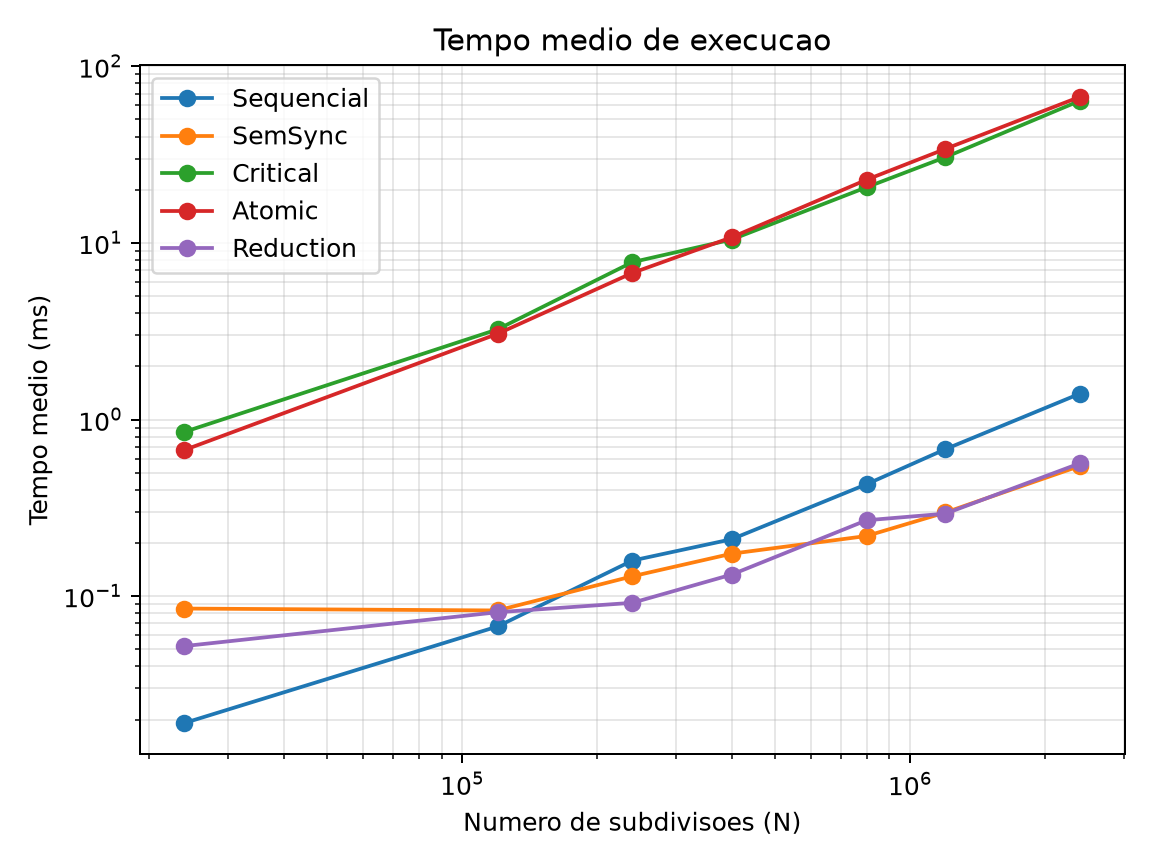
\includegraphics[
        width=0.90\textwidth
    ]{../ATVD6/tempo_medio.png}

    \caption{Tempo médio de execução em função do número de subdivisões.}
    \label{fig:atvd06-tempo}
\end{figure}

A escala logarítmica no eixo dos tempos permite visualizar simultaneamente
implementações com diferenças superiores a uma ordem de grandeza.

\texttt{Critical} e \texttt{Atomic} apresentam crescimento elevado,
enquanto Sequencial e \texttt{Reduction} permanecem em uma região
consideravelmente inferior.


\subsection{Speedup}

\begin{figure}[htbp]
    \centering
    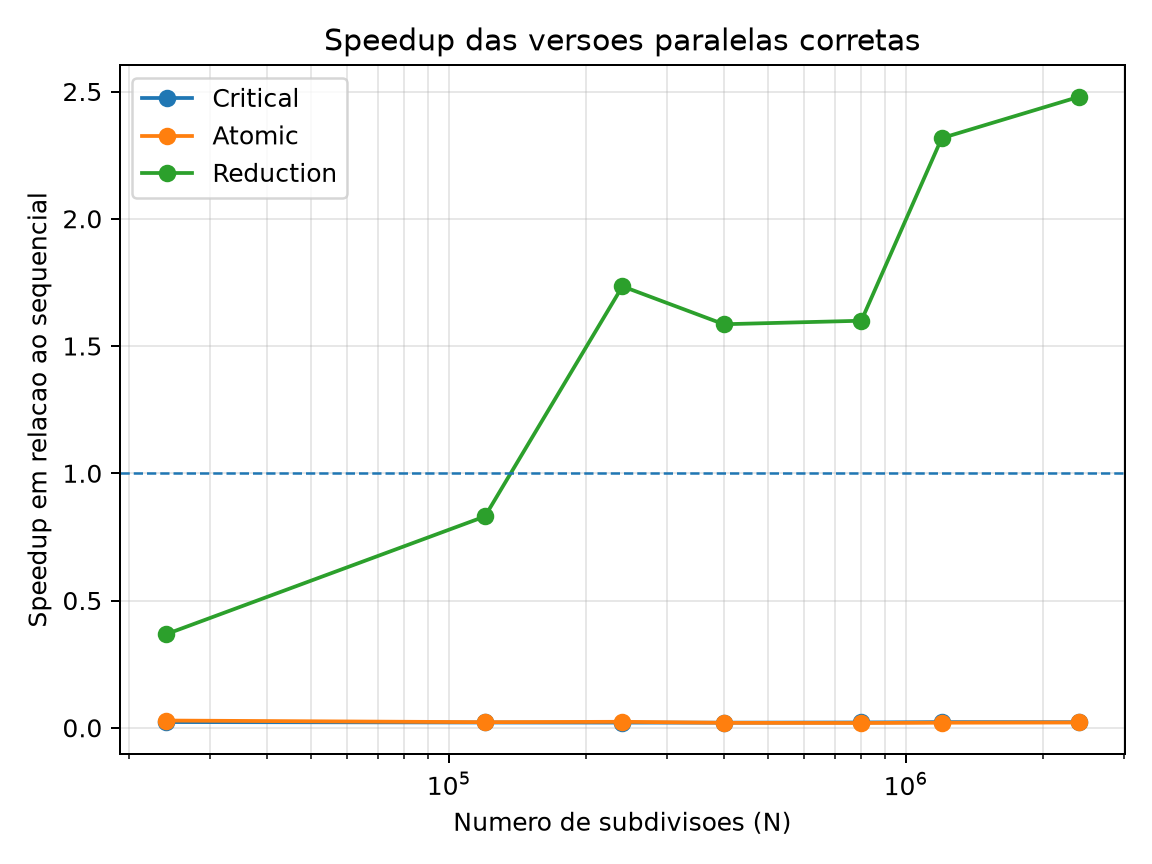
\includegraphics[
        width=0.90\textwidth
    ]{../ATVD6/speedup.png}

    \caption{Speedup das estratégias paralelas funcionalmente válidas.}
    \label{fig:atvd06-speedup}
\end{figure}

A linha \(S=1\) representa o desempenho do baseline sequencial.

\texttt{Critical} e \texttt{Atomic} permanecem abaixo desse limite em todas
as configurações.

\texttt{Reduction} ultrapassa a referência a partir da região entre
\(N=24\,000\) e \(N=120\,000\), tornando o ganho mais evidente nos tamanhos
posteriores.


\subsection{Erro absoluto médio}

\begin{figure}[htbp]
    \centering
    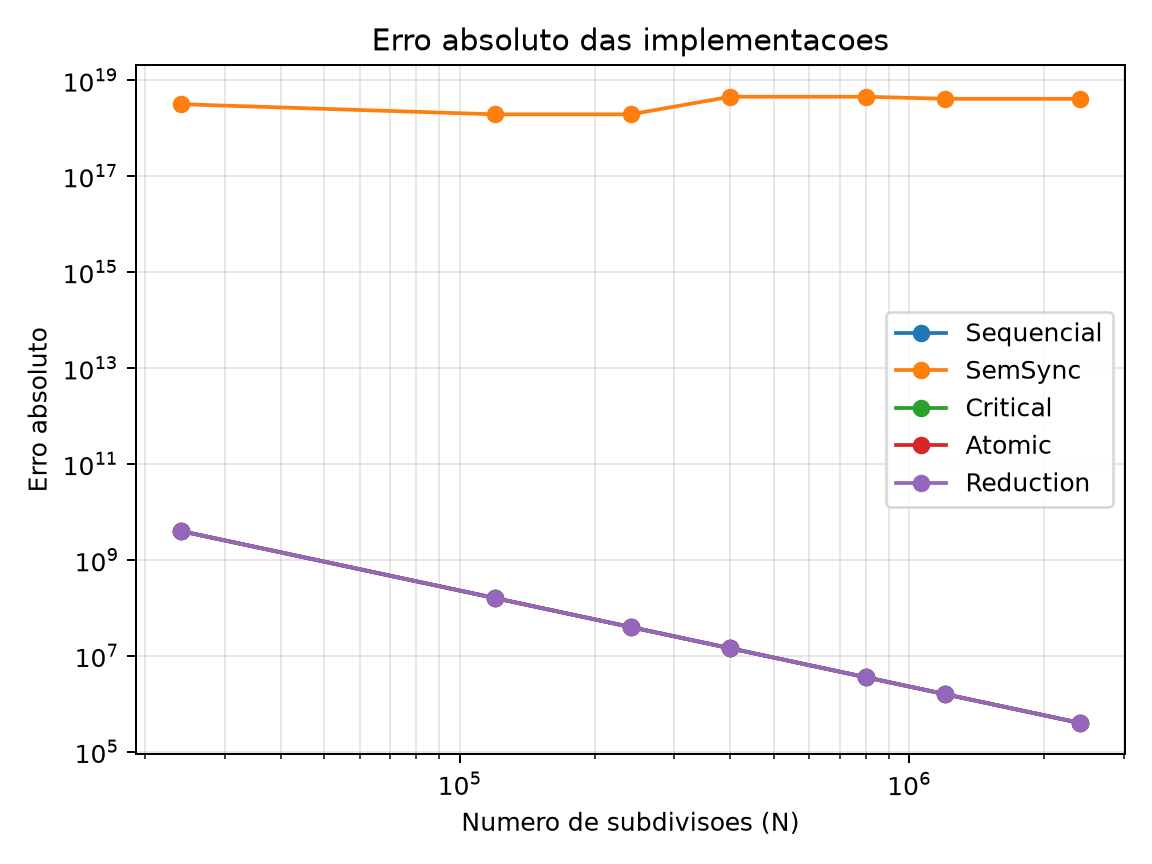
\includegraphics[
        width=0.90\textwidth
    ]{../ATVD6/erro_absoluto.png}

    \caption{Erro absoluto médio das implementações.}
    \label{fig:atvd06-erro}
\end{figure}

Sequencial, \texttt{Critical}, \texttt{Atomic} e \texttt{Reduction}
produzem exatamente os mesmos erros e, portanto, suas curvas se sobrepõem.

A curva de \texttt{SemSync} permanece várias ordens de grandeza acima,
evidenciando o impacto da race condition sobre a correção do resultado.


\section{Análise e discussão}

\label{sec:atvd06-discussao}

\subsection{Impacto da ausência de sincronização}

A versão sem sincronização mostrou diretamente a necessidade de proteger a
operação de redução.

Para \(N=24\,000\), apenas

\begin{equation}
    4/20
\end{equation}

execuções foram corretas.

Para todos os demais valores:

\begin{equation}
    0/20
\end{equation}

resultados foram válidos.

O erro absoluto médio permaneceu na ordem de

\begin{equation}
    10^{18},
\end{equation}

enquanto as versões corretas apresentaram erro determinado apenas pela
discretização do método.

O resultado demonstra que simplesmente distribuir as iterações não é
suficiente: a semântica da atualização compartilhada precisa ser preservada.


\subsection{Desempenho de \texttt{critical}}

A versão \texttt{Critical} garantiu

\begin{equation}
    20/20
\end{equation}

resultados corretos em todas as configurações.

Entretanto, apresentou o maior custo de sincronização.

Para

\begin{equation}
    N=2\,400\,000,
\end{equation}

foram obtidos

\begin{equation}
    T_{\text{seq}}
    =
    1.874432\ \text{ms}
\end{equation}

e

\begin{equation}
    T_{\text{critical}}
    =
    92.877570\ \text{ms}.
\end{equation}

A razão é aproximadamente

\begin{equation}
    \frac{92.877570}{1.874432}
    \approx
    49.5.
\end{equation}

Assim, nessa configuração, a versão \texttt{Critical} foi aproximadamente
\(49.5\) vezes mais lenta que a sequencial.

O speedup correspondente foi

\begin{equation}
    S_{\text{critical}}
    =
    0.020.
\end{equation}

A explicação está na serialização de cada atualização do acumulador. Embora
o cálculo de \(x_i\) e \(f(x_i)\) ocorra em paralelo, todas as threads
precisam entrar repetidamente na mesma região de exclusão mútua.


\subsection{Desempenho de \texttt{atomic}}

A implementação \texttt{Atomic} também produziu resultados corretos em
todas as medições.

Na execução final, foi mais rápida que \texttt{Critical} em todos os valores
de \(N\).

Para

\begin{equation}
    N=2\,400\,000,
\end{equation}

o tempo foi

\begin{equation}
    T_{\text{atomic}}
    =
    61.214450\ \text{ms}.
\end{equation}

Comparando com \texttt{Critical}:

\begin{equation}
    \frac{92.877570}{61.214450}
    \approx
    1.52.
\end{equation}

Apesar dessa melhoria, o speedup em relação ao sequencial foi apenas

\begin{equation}
    S_{\text{atomic}}
    =
    0.031.
\end{equation}

Portanto, \texttt{atomic} reduz o custo em relação a uma região crítica
genérica, mas não elimina o gargalo principal.

Todas as threads ainda executam uma operação de leitura-modificação-escrita
sobre o mesmo acumulador.

Esse padrão produz contenção e tráfego de coerência sobre o mesmo endereço
de memória.


\subsection{Desempenho de \texttt{reduction}}

A implementação utilizando \texttt{reduction} apresentou o melhor
comportamento entre as estratégias paralelas corretas.

Para \(N=24\,000\):

\begin{equation}
    S_{\text{reduction}}
    =
    0.304.
\end{equation}

Portanto, o problema ainda era pequeno demais para compensar o overhead do
OpenMP.

Para \(N=120\,000\):

\begin{equation}
    S_{\text{reduction}}
    =
    1.015,
\end{equation}

indicando desempenho praticamente equivalente ao sequencial.

A partir de \(N=240\,000\), o ganho tornou-se mais evidente:

\begin{equation}
    S_{\text{reduction}}
    =
    1.509.
\end{equation}

Para \(N=400\,000\):

\begin{equation}
    S_{\text{reduction}}
    =
    2.014.
\end{equation}

O maior speedup observado ocorreu para

\begin{equation}
    N=1\,200\,000,
\end{equation}

com

\begin{equation}
    \boxed{
        S_{\text{reduction}}=2.716
    }.
\end{equation}

Com quatro threads, a eficiência correspondente é

\begin{equation}
    E_4
    =
    \frac{2.716}{4}
    \approx
    0.679,
\end{equation}

ou aproximadamente

\begin{equation}
    \boxed{67.9\%}.
\end{equation}


\subsection{Comportamento no maior valor de \(N\)}

Para

\begin{equation}
    N=2\,400\,000,
\end{equation}

o tempo sequencial foi

\begin{equation}
    1.874432\ \text{ms},
\end{equation}

enquanto \texttt{Reduction} apresentou

\begin{equation}
    0.875025\ \text{ms}.
\end{equation}

O speedup foi

\begin{equation}
    S=2.142.
\end{equation}

Esse valor é inferior ao máximo de \(2.716\) observado para
\(N=1\,200\,000\).

O speedup real não precisa crescer monotonicamente com \(N\). Entre os
fatores que podem afetar a relação estão:

\begin{itemize}
    \item escalonamento do sistema operacional;
    \item frequência dinâmica do processador;
    \item estado térmico;
    \item comportamento de cache;
    \item overhead do runtime OpenMP.
\end{itemize}

Mesmo com essa redução no último ponto, a implementação permaneceu mais de
duas vezes mais rápida que o baseline sequencial.


\subsection{Granularidade}

Os resultados demonstram a importância da granularidade.

Para cargas pequenas, o custo de:

\begin{itemize}
    \item iniciar a região paralela;
    \item distribuir iterações;
    \item sincronizar a equipe;
    \item combinar os acumuladores;
\end{itemize}

é comparável ou superior ao trabalho útil.

Isso explica

\begin{equation}
    S<1
\end{equation}

para \texttt{Reduction} em \(N=24\,000\).

À medida que \(N\) cresce, uma quantidade maior de trabalho é distribuída
entre as threads e o overhead fixo é progressivamente amortizado.


\subsection{Correção versus desempenho}

Os resultados também demonstram que desempenho não pode ser avaliado
isoladamente.

Em diversas configurações, \texttt{SemSync} apresenta tempo inferior ao
sequencial. Por exemplo, em \(N=1\,200\,000\), o valor temporal calculado
corresponde a um fator de

\begin{equation}
    2.617
\end{equation}

em relação ao sequencial.

Entretanto:

\begin{equation}
    0/20
\end{equation}

resultados foram corretos.

Portanto, esse valor não pode ser interpretado como speedup de uma solução
válida.

A comparação evidencia a seguinte relação:

\begin{center}
\begin{tabular}{l|c|c}
    \hline
    Estratégia & Correção & Desempenho observado \\
    \hline
    Sequencial & sim & baseline \\
    SemSync & não & não utilizável \\
    Critical & sim & fortemente degradado \\
    Atomic & sim & degradado por contenção \\
    Reduction & sim & melhor estratégia paralela \\
    \hline
\end{tabular}
\end{center}


\subsection{Por que \texttt{reduction} apresenta melhor escalabilidade}

Em \texttt{critical} e \texttt{atomic}, todas as threads atualizam
continuamente a mesma posição de memória.

Em \texttt{reduction}, cada thread mantém sua soma privada durante a maior
parte da execução.

Conceitualmente:

\begin{figure}[htbp]
    \centering
    \begin{tikzpicture}[node distance=0.65cm and 0.65cm, font=\small]
        \node[processo, text width=4.4cm] (iterations)
            {Iterações do laço};
        \node[thread, below left=of iterations, text width=2.7cm] (t1)
            {Thread 1};
        \node[thread, below=of iterations, text width=2.7cm] (t2)
            {Thread 2};
        \node[thread, below right=of iterations, text width=2.7cm] (tp)
            {Thread \(P\)};
        \node[componente, below=of t1, text width=2.7cm] (s1)
            {Soma privada \(S_1\)};
        \node[componente, below=of t2, text width=2.7cm] (s2)
            {Soma privada \(S_2\)};
        \node[componente, below=of tp, text width=2.7cm] (sp)
            {Soma privada \(S_P\)};
        \node[processo, below=1.0cm of s2, text width=3.5cm] (reduction)
            {Redução final};
        \node[componente, below=of reduction, text width=2.7cm] (total)
            {Soma total \(S\)};
        \draw[fluxo] (iterations) -- (t1);
        \draw[fluxo] (iterations) -- (t2);
        \draw[fluxo] (iterations) -- (tp);
        \draw[fluxo] (t1) -- (s1);
        \draw[fluxo] (t2) -- (s2);
        \draw[fluxo] (tp) -- (sp);
        \draw[fluxo] (s1) |- (reduction);
        \draw[fluxo] (s2) -- (reduction);
        \draw[fluxo] (sp) |- (reduction);
        \draw[fluxo] (reduction) -- (total);
    \end{tikzpicture}

    \caption{Estratégia conceitual utilizada pela redução.}
    \label{fig:atvd06-reduction}
\end{figure}

A sincronização deixa de ocorrer em cada iteração e passa a ser concentrada
na combinação final dos resultados parciais.

Essa propriedade explica o desempenho significativamente superior observado
experimentalmente.


\section{Limitações}

\label{sec:atvd06-limitacoes}

O experimento possui algumas limitações que devem ser consideradas na
interpretação dos resultados.

Primeiramente, somente quatro threads foram avaliadas. Portanto, a atividade
permite comparar estratégias de sincronização para uma configuração fixa,
mas não caracteriza a escalabilidade em função do número de threads.

Também foi utilizada apenas a função

\begin{equation}
    f(x)=x^2,
\end{equation}

cujo custo computacional é pequeno e uniforme. Funções mais complexas podem
alterar significativamente a razão entre trabalho útil e overhead de
sincronização.

O uso de \texttt{schedule(static)} é adequado à uniformidade dessa carga,
mas os resultados não caracterizam problemas com custo variável por
iteração.

A aritmética inteira com \texttt{int64\_t} evita erros de ponto flutuante e
facilita a validação. Entretanto, muitas aplicações reais de integração
numérica utilizam \texttt{double}, situação em que a ordem de redução também
pode introduzir pequenas diferenças de arredondamento.

A compilação desabilita a vetorização automática com
\texttt{-fno-tree-vectorize}. Dessa forma, a comparação prioriza os efeitos
de OpenMP e sincronização, não o máximo desempenho disponível com SIMD.

Os atributos \texttt{noinline} e \texttt{noipa} são utilizados para
preservar o trabalho que deve ser medido. Essa decisão é metodologicamente
necessária ao benchmark, mas restringe algumas otimizações que poderiam
ocorrer em um programa de produção.

O batching adaptativo utiliza uma execução piloto para estimar o tamanho do
lote. Flutuações nessa medição podem resultar em lotes cuja duração real
posterior se afasta do alvo de 20 ms. Esse efeito foi especialmente visível
em algumas medições da versão \texttt{SemSync}, cuja execução também é
afetada pela própria condição de corrida.

A versão sem sincronização contém deliberadamente uma race condition.
Consequentemente, seus resultados não são determinísticos e não representam
uma implementação funcionalmente válida.

Por fim, os experimentos foram executados em sistema operacional de
propósito geral. Escalonamento, serviços em segundo plano, frequência
dinâmica e estado térmico podem provocar variações entre execuções.


\section{Conclusões da atividade}

\label{sec:atvd06-conclusao}

A Atividade 6 permitiu avaliar experimentalmente quatro formas distintas de
tratar a dependência sobre o acumulador do método composto do trapézio.

A versão sem sincronização demonstrou diretamente a consequência de uma race
condition. Em \(N=24\,000\), somente quatro das vinte medições produziram o
resultado esperado, enquanto todos os tamanhos posteriores apresentaram
zero resultados válidos em vinte execuções.

A diretiva \texttt{critical} restaurou a correção, porém introduziu forte
serialização. No maior tamanho analisado, essa versão foi aproximadamente
\(49.5\) vezes mais lenta que a execução sequencial.

A diretiva \texttt{atomic} reduziu o custo em relação a
\texttt{critical}, mas continuou apresentando forte contenção sobre o mesmo
acumulador compartilhado. Para \(N=2\,400\,000\), seu speedup foi apenas
\(0.031\).

A versão baseada em \texttt{reduction} apresentou o melhor equilíbrio entre
correção e desempenho. Para problemas pequenos, seu overhead superou o
benefício do paralelismo. Com o crescimento de \(N\), entretanto, o trabalho
paralelo passou a amortizar esse custo.

O maior speedup observado foi

\begin{equation}
    \boxed{2.716}
\end{equation}

com quatro threads em

\begin{equation}
    N=1\,200\,000,
\end{equation}

correspondendo a eficiência aproximada de

\begin{equation}
    \boxed{67.9\%}.
\end{equation}

Os resultados demonstram que a mera introdução de múltiplas threads não
garante ganho de desempenho. A estratégia utilizada para coordenar os dados
compartilhados é determinante.

Para o padrão de soma presente no método do trapézio, a redução mostrou-se
substancialmente mais adequada que a proteção do acumulador em cada
iteração.


\section{Síntese}

\label{sec:atvd06-defesa}

Os principais pontos para defesa oral podem ser sintetizados da seguinte
forma:

\begin{enumerate}

    \item A Atividade 6 implementa experimentalmente a paralelização que havia
    sido discutida teoricamente na Atividade 4.

    \item O problema matemático foi mantido:
    \[
        f(x)=x^2,
        \qquad
        [a,b]=[0,2\,400\,000].
    \]

    \item Foram comparadas cinco versões:
    Sequencial, SemSync, Critical, Atomic e Reduction.

    \item Todas as versões executam exatamente o mesmo cálculo; a principal
    diferença é a forma como o acumulador \texttt{soma} é tratado.

    \item Foram utilizadas quatro threads e
    \texttt{schedule(static)}.

    \item O escalonamento estático foi escolhido porque todas as iterações
    possuem custo aproximadamente uniforme.

    \item Foram realizados três aquecimentos e vinte medições por
    configuração.

    \item Foi utilizado batching adaptativo com alvo de aproximadamente
    20 ms, porque uma quantidade fixa de repetições seria inadequada para
    versões com custos muito diferentes.

    \item O tempo apresentado corresponde à média das vinte medições,
    conforme solicitado pelo enunciado.

    \item A versão SemSync possui uma race condition no acumulador.

    \item Em \(N=24\,000\), SemSync produziu apenas 4 resultados corretos em
    20 medições; para todos os demais valores, produziu 0/20.

    \item O erro de SemSync é apresentado como erro absoluto médio das vinte
    medições, e não como erro de uma única execução.

    \item Critical resolve a race condition, mas serializa cada atualização
    da soma.

    \item No maior caso, Critical demorou aproximadamente 92.88 ms contra
    1.87 ms do sequencial, sendo cerca de 49.5 vezes mais lento.

    \item Atomic também garante correção e foi mais rápido que Critical na
    execução final, porém todas as threads continuam disputando o mesmo
    acumulador.

    \item No maior caso, Atomic apresentou speedup de apenas
    \[
        0.031.
    \]

    \item Reduction utiliza acumuladores privados e combina os resultados ao
    final, evitando sincronização sobre a soma em cada iteração.

    \item Para \(N=24\,000\), Reduction ainda foi mais lenta que o
    sequencial:
    \[
        S=0.304.
    \]

    \item Em \(N=120\,000\), o desempenho ficou praticamente no ponto de
    equilíbrio:
    \[
        S=1.015.
    \]

    \item A partir dos tamanhos seguintes, Reduction passou a apresentar
    ganho consistente.

    \item O maior speedup observado foi
    \[
        S=2.716
    \]
    para
    \[
        N=1\,200\,000.
    \]

    \item Com quatro threads, isso corresponde a eficiência de
    aproximadamente
    \[
        67.9\%.
    \]

    \item O speedup não cresceu monotonicamente: em
    \(N=2\,400\,000\), Reduction apresentou
    \[
        S=2.142.
    \]
    Essa variação é compatível com fatores reais de execução como runtime
    OpenMP, escalonamento, frequência dinâmica e estado do sistema.

    \item O aparente speedup da versão SemSync não deve ser interpretado como
    ganho válido, pois desempenho sem correção funcional não representa uma
    solução utilizável.

    \item A principal conclusão é que, para uma soma paralela, proteger cada
    atualização com Critical ou Atomic pode introduzir contenção suficiente
    para tornar o programa muito mais lento.

    \item Para esse padrão computacional, Reduction foi a estratégia que
    melhor preservou simultaneamente correção e desempenho.

\end{enumerate}
